\documentclass[conference]{IEEEtran}
\IEEEoverridecommandlockouts

\usepackage{amsmath,amssymb,amsfonts}
\usepackage{algorithmic}
\usepackage{graphicx}
\usepackage{textcomp}
\usepackage{xcolor}
\usepackage{booktabs}
\usepackage{cite}
\usepackage{microtype}
\usepackage{url}
\usepackage{enumitem}
\usepackage{balance}

\graphicspath{{figures/}}

% Optimal float placement & compact spacing
\renewcommand{\topfraction}{0.95}
\renewcommand{\bottomfraction}{0.95}
\renewcommand{\textfraction}{0.05}
\renewcommand{\floatpagefraction}{0.85}
\renewcommand{\dbltopfraction}{0.95}
\renewcommand{\dblfloatpagefraction}{0.85}

\setlength{\textfloatsep}{4pt plus 1pt minus 1pt}
\setlength{\floatsep}{4pt plus 1pt minus 1pt}
\setlength{\intextsep}{4pt plus 1pt minus 1pt}
\setlength{\abovecaptionskip}{2pt plus 1pt minus 1pt}
\setlength{\belowcaptionskip}{2pt plus 1pt minus 1pt}
\setlength{\dbltextfloatsep}{4pt plus 1pt minus 1pt}
\setlength{\dblfloatsep}{4pt plus 1pt minus 1pt}
\renewcommand{\arraystretch}{0.90}

% Compact list spacing
\setlist{itemsep=0.5pt, topsep=1.0pt, parsep=0pt, leftmargin=*}

% Compact bibliography spacing
\let\oldthebibliography\thebibliography
\let\endoldthebibliography\endthebibliography
\renewenvironment{thebibliography}[1]{%
  \begin{oldthebibliography}{#1}%
    \setlength{\itemsep}{0pt}%
    \setlength{\parskip}{0pt}%
}{%
  \end{oldthebibliography}%
}

\begin{document}

\title{When Is Algorithm Selection Worth the Cost?\\ An Overhead-Aware Study of Exact Shortest-Path Computation}

\author{
\IEEEauthorblockN{Ganeshvar K S}
\IEEEauthorblockA{\textit{School of Computer Science} \\
\textit{Vellore Institute of Technology}\\
Chennai, India}
\and
\IEEEauthorblockN{Sai Siddaarth}
\IEEEauthorblockA{\textit{School of Computer Science} \\
\textit{Vellore Institute of Technology}\\
Chennai, India}
\and
\IEEEauthorblockN{Uma Maheshwari}
\IEEEauthorblockA{\textit{School of Computer Science} \\
\textit{Vellore Institute of Technology}\\
Chennai, India}
}

\maketitle

\begin{abstract}
Per-instance algorithm selection is usually evaluated on the assumption that feature extraction and model inference are negligible next to solver execution. That assumption holds for satisfiability or integer programming, where single runs take seconds, but it is questionable for single-pair exact shortest-path queries on small and moderate graphs, which finish in hundreds of microseconds. This paper asks when adaptive shortest-path solver selection can pay for its own decision cost. We charge graph-level features, query-level features, feature-vector assembly, and selector inference against the Single-Best-Solver (SBS) to Virtual-Best-Solver (VBS) oracle gap, and we summarize viability with the break-even ratio $\mathrm{RequiredCapture}(Q)$ and the zero-overhead decision-quality measure $\mathrm{SolverOnlyCapture}(Q)$: adaptive selection beats the fixed policy exactly when the latter exceeds the former. The study covers 48 synthetic graphs from three families (Erd\H{o}s--R\'enyi, random geometric, Barab\'asi--Albert; $V \in \{40,80,160,320\}$, $D \in \{6,12\}$), 500 deterministic queries per graph, checkpoints $Q \in \{1,10,50,100,500\}$, and a portfolio of Dijkstra, Bidirectional Dijkstra, and $A^*$. Measured per-query inference is $87.9\,\mu\mathrm{s}$ under library inference and $0.8\,\mu\mathrm{s}$ when the decision tree is compiled to native branches ($\approx 110\times$). At $Q=500$, $\mathrm{RequiredCapture} = 3.8527$ in library mode, so overhead exceeds the entire oracle gap and no selector could break even; compiling lowers it to $0.2898$, within the affordable range. Decision quality then binds: $\mathrm{SolverOnlyCapture} = -0.1633$, and after qualifying differences against empirical pass-to-pass dispersion ($16.32\%$ library, $9.40\%$ compiled), none of the 40 evaluated graph--workload cells shows a genuine crossover. Solver complementarity is nevertheless present: in geometric graphs, $A^*$ attains the per-query runtime minimum on $6\%$--$20\%$ of queries. Within the evaluated envelope, the conventional classifier does not convert this complementarity into a genuine task-level speedup, which points to the selection objective rather than the absence of exploitable structure as the remaining obstacle.
\end{abstract}

\begin{IEEEkeywords}
Algorithm selection, shortest-path algorithms, overhead accounting, empirical algorithmics, runtime profiling.
\end{IEEEkeywords}

\section{Introduction}

Single-pair exact shortest-path computation is a standard primitive in network routing, transportation planning, geographic information retrieval, and graph analytics \cite{dijkstra1959, bast2016}. Several exact algorithms are available for the same query, and none of them dominates. Dijkstra's algorithm \cite{dijkstra1959} expands an isotropic frontier from the source. Bidirectional Dijkstra \cite{nicholson1966, pohl1971} expands two frontiers that meet in the middle, which reduces the explored region on many instances. $A^*$ \cite{hart1968} steers expansion toward the target with an admissible heuristic whenever the graph carries an embedding that supports one.

Which solver is fastest therefore varies with topology, size, density, and query placement. Section~\ref{sec:complementarity} measures this variability directly: on the random geometric graphs used here, the per-query winner is Bidirectional Dijkstra on $37.8\%$--$66.8\%$ of queries, Dijkstra on $23.4\%$--$50.4\%$, and $A^*$ on $5.6\%$--$19.6\%$. Instance-level complementarity of this kind is the precondition for any selection scheme to be useful.

Per-instance algorithm selection, formulated by Rice \cite{rice1976}, exploits such complementarity by mapping instance features to the solver predicted to run fastest on that instance. Portfolio systems for satisfiability and related problems, including SATzilla \cite{xu2008}, ASlib \cite{bischl2016}, LLAMA \cite{kotthoff2014}, claspfolio 2 \cite{gebser2014}, and AutoFolio \cite{lindauer2015}, have produced large gains in settings where single runs last seconds or longer. In those settings the cost of computing features and evaluating a model is absorbed by the runtime it is trying to reduce, and the survey of Kerschke et al.\ \cite{kerschke2019} lists feature cost among the practical issues that selection systems must handle.

This cost structure does not transfer automatically to high-throughput graph workloads. Exact shortest-path queries on graphs with a few hundred vertices complete in hundreds of microseconds. A selector that reads a handful of features, assembles a feature vector, and evaluates a decision tree before dispatch pays a price that is comparable to the work it is scheduling. Part of the cost is one-time and can be amortized over a resident graph serving $Q$ queries; per-query features and inference recur on every query and cannot.

The literature characterizes shortest-path solver behavior across graph landscapes \cite{gholami2026} and analyzes feature-computation budgets for per-instance selection in black-box optimization \cite{vanderblom2026}. Neither line of work prices the complete decision -- graph characterization, per-query features, vector assembly, and inference -- against the performance headroom actually available on a repeated-query shortest-path workload. That price is what determines whether adaptive selection is economically viable, and it is the subject of this paper. We ask:

\begin{quote}
\emph{Within what graph and query-workload boundaries can adaptive exact shortest-path algorithm selection capture enough SBS--VBS headroom to amortize its feature-extraction and inference overhead?}
\end{quote}

To answer it, we study an overhead-priced pipeline (Features $\rightarrow$ Selector inference $\rightarrow$ Solver execution) and charge every measured component of the decision against the empirical gap between the Single Best Solver (SBS) and the Virtual Best Solver (VBS). The study is an empirical characterization, not a new solver or a new learning architecture; its contribution is the accounting discipline and the boundary conditions that the accounting exposes.

\subsection*{Contributions}
\begin{enumerate}
    \item \textbf{Overhead-priced selection model.} We decompose adaptive execution into graph features, query features, feature-vector assembly, selector inference, and selected-solver execution, all measured in the same loop as the workload (Section~\ref{sec:cost}).
    \item \textbf{Break-even accounting criterion.} We define $\mathrm{RequiredCapture}(Q) = \mathrm{SelectionOverhead}(Q)/\mathrm{OracleGap}(Q)$ and show that net viability is equivalent to $\mathrm{SolverOnlyCapture}(Q) > \mathrm{RequiredCapture}(Q)$; the criterion separates overhead from decision quality instead of merging them.
    \item \textbf{Workload-amortization analysis.} We measure the economics at $Q \in \{1,10,50,100,500\}$ on 48 graphs, isolating the point at which one-time graph characterization stops dominating and recurring per-query costs take over.
    \item \textbf{Library versus compiled deployment.} We compare out-of-the-box \texttt{scikit-learn} single-row inference with a decision tree compiled to native conditional branches. Compilation reduces per-query inference from $87.9\,\mu\mathrm{s}$ to $0.8\,\mu\mathrm{s}$ and moves selection from $\mathrm{RequiredCapture} = 3.8527$ to $0.2898$ at $Q=500$.
    \item \textbf{Solver-complementarity diagnostics.} We report per-query winner shares per graph family, which quantify how much headroom exists for a selector to exploit in the first place.
    \item \textbf{Runtime-regret interpretation.} We show that the residual bottleneck after compilation is the training objective: unweighted $0/1$ classification treats a cheap misprediction and an expensive one alike, and the resulting selector captures no net solver-side savings.
    \item \textbf{Reproducible protocol.} The study uses deterministic generation, a frozen split manifest, SHA-256 integrity checks, and an automated audit of 15 conditions over the raw records; all reported quantities are recomputable from the frozen artifacts (Section~\ref{sec:repro}).
\end{enumerate}

\section{Related Work}

\subsection{Algorithm Selection and Empirical Algorithmics}
Rice \cite{rice1976} formalized per-instance algorithm selection as a mapping from instance features to algorithms, with performance measured on a distribution of instances. In combinatorial search, portfolio systems such as SATzilla \cite{xu2008, hutter2014} predict solver runtimes or solve probabilities for SAT; ASlib \cite{bischl2016} standardized benchmarking and introduced the SBS and VBS reference policies we adopt here; LLAMA \cite{kotthoff2014}, claspfolio 2 \cite{gebser2014}, and AutoFolio \cite{lindauer2015} automated portfolio construction and configuration for constraint-satisfaction problems. Kerschke et al.\ \cite{kerschke2019} survey the area and identify feature computation as a recurring practical cost. Hutter et al.\ \cite{hutter2014} study runtime prediction directly, which is the objective family our results point back to when classification quality and runtime quality diverge. This literature assumes, and sometimes explicitly checks, that per-instance runtimes are long enough for feature and inference costs to be a small fraction of the quantity being optimized.

\subsection{Feature-Cost and Budget-Aware Selection}
The cost of features has been analyzed for per-instance selection in black-box optimization by van der Blom and Vermetten \cite{vanderblom2026}, who charge landscape-analysis features against a fixed evaluation budget and identify budget fractions that maximize performance. Our work shares the premise that selection must justify its characterization cost, and we make no claim of novelty for feature-cost awareness in general. The setting and measurement differ in three respects. First, cost dimension: they charge sampling-based features against an internal optimization budget, whereas we price wall-clock feature extraction and selector inference in a deployed pipeline. Second, workload structure: black-box optimization instances are evaluated in isolation, whereas shortest-path workloads query a resident graph repeatedly, which introduces workload size $Q$ as an explicit amortization axis for one-time graph characterization. Third, the accounting device: we compare measured decision cost to measured headroom through a break-even ratio, which yields the overhead-bound and efficacy-bound regimes reported in Section~\ref{sec:d}.

\subsection{Shortest-Path Solvers and Instance Landscapes}
Algorithm engineering has produced many exact point-to-point techniques beyond the textbook algorithms: Dijkstra's priority-queue method \cite{dijkstra1959}, bidirectional search \cite{nicholson1966, pohl1971}, $A^*$ \cite{hart1968}, landmark-based ALT \cite{goldberg2005}, and hierarchical approaches such as contraction hierarchies and transit-node routing used in routing engines \cite{bast2016}. Our portfolio deliberately uses three textbook solvers so that the measured headroom reflects algorithmic diversity that a small selector can plausibly exploit. Closest to our setting is the recent landscape study of Gholami Shiri et al.\ \cite{gholami2026}, which embeds graphs in a structural feature space, clusters them into landscape regions, and compares runtime distributions of Dijkstra, Bidirectional Dijkstra, $A^*$, and DEQ on weighted random, geometric, and road networks. That work establishes that structural similarity relates to solver performance; it does not implement a selector, charge feature or inference cost, expose a workload-amortization axis, or compute oracle headroom. Our study examines the operational question their analysis motivates: given that the solvers differ by instance, does exploiting the difference repay the cost of the decision -- and where does the answer change between deployment modes?

\section{Cost Model and Evaluation Framework}
\label{sec:cost}

\subsection{Selection Setting}
Let $G=(V,E,w)$ be a weighted undirected graph with non-negative edge weights $w:E \to \mathbb{R}^{+}$. A query $q=(s,t)$ requests the exact minimum-weight path between $s \in V$ and $t \in V$. A portfolio $\mathcal{A}=\{A_1,\dots,A_m\}$ contains exact solvers, and $t(A;G,q)$ denotes the wall-clock time solver $A$ needs to return the optimal distance $d^{*}(s,t)$. An adaptive selector $S:\Phi(G,q) \to \mathcal{A}$ maps a feature vector $\Phi(G,q)$ to a solver. All selector features in this study are computed from graph metadata, edge weights, and query endpoints before the selected solver runs; Section~\ref{sec:features} states this requirement explicitly and lists the features.

\subsection{Reference Policies: SBS and VBS}
Following standard empirical-algorithmics practice \cite{bischl2016}, we compare against two reference policies. The \textbf{Single Best Solver (SBS)} is the fixed solver that minimizes cumulative runtime on the training distribution $\mathcal{D}_{\mathrm{train}}$:
\begin{equation}
A_{\mathrm{SBS}} = \arg\min_{A \in \mathcal{A}} \sum_{(G,q) \in \mathcal{D}_{\mathrm{train}}} t(A;G,q).
\end{equation}
The \textbf{Virtual Best Solver (VBS)} is a zero-overhead per-query oracle that runs the fastest eligible solver for each instance:
\begin{equation}
t(\mathrm{VBS};G,q) = \min_{A \in \mathcal{A}_{\mathrm{elig}}(G,q)} t(A;G,q),
\end{equation}
where $\mathcal{A}_{\mathrm{elig}}(G,q) \subseteq \mathcal{A}$ is the set of solvers eligible for that instance. VBS is a lower bound on solver execution time, not an implementable policy, because deciding which solver is fastest would require running them.

\subsection{Oracle Gap and Capture Rate}
For a workload of $Q$ queries on graph $G$, let $C_{\mathrm{SBS}}(Q)=\sum_{i=1}^{Q} t(A_{\mathrm{SBS}};G,q_i)$ and $C_{\mathrm{VBS}}(Q)=\sum_{i=1}^{Q} t(\mathrm{VBS};G,q_i)$. The available performance headroom is the oracle gap:
\begin{equation}
\mathrm{OracleGap}(Q) = C_{\mathrm{SBS}}(Q) - C_{\mathrm{VBS}}(Q).
\end{equation}
No selector can save more than $\mathrm{OracleGap}(Q)$ on that workload, whatever its accuracy. Writing $C_{\mathrm{Adaptive}}(Q)$ for the total cost of the adaptive pipeline, the \textbf{Capture Rate} expresses realized performance relative to that gap:
\begin{equation}
\mathrm{CaptureRate}(Q) = \frac{C_{\mathrm{SBS}}(Q) - C_{\mathrm{Adaptive}}(Q)}{C_{\mathrm{SBS}}(Q) - C_{\mathrm{VBS}}(Q)}.
\end{equation}
A value of $1.0$ would match the oracle, $0.0$ denotes parity with the fixed policy, and negative values mean that adaptive selection is slower than simply running the SBS.

\subsection{Selection Overhead, Required Capture, and Solver-Only Capture}
The adaptive cost decomposes into a one-time graph characterization, recurring per-query feature extraction, feature-vector assembly, selector inference, and the selected solver:
\begin{equation}
\begin{aligned}
C_{\mathrm{Adaptive}}(Q) &= C_{\mathrm{feat}}^{\mathrm{graph}}(G) + \sum_{i=1}^{Q}\Bigl[ C_{\mathrm{feat}}^{\mathrm{query}}(G,q_i) \\
&\quad + C_{\mathrm{vec}}(q_i) + C_{\mathrm{sel}}(q_i) + t(S(\Phi);G,q_i)\Bigr].
\end{aligned}
\end{equation}
Grouping the terms that exist only because a decision is made gives the selection overhead:
\begin{equation}
\begin{aligned}
\mathrm{SelectionOverhead}(Q) ={}& C_{\mathrm{feat}}^{\mathrm{graph}}(G) \\
&{}+ \sum_{i=1}^{Q}\bigl[ C_{\mathrm{feat}}^{\mathrm{query}}(G,q_i) \\
&{}\qquad + C_{\mathrm{vec}}(q_i) + C_{\mathrm{sel}}(q_i)\bigr].
\end{aligned}
\end{equation}
The \textbf{Required Capture} is the fraction of the oracle gap that a selector must capture to pay for its own decision cost:
\begin{equation}
\mathrm{RequiredCapture}(Q) = \frac{\mathrm{SelectionOverhead}(Q)}{\mathrm{OracleGap}(Q)} .
\end{equation}
The interpretation is a break-even statement. If $\mathrm{RequiredCapture}(Q) > 1$, the decision costs more than the entire available headroom, so even an omniscient selector that always picks the oracle solver would still lose to the fixed policy. If $\mathrm{RequiredCapture}(Q) < 1$, overhead is affordable in principle, and the remaining question is whether the selector captures enough headroom. To separate overhead from decision quality we also report the \textbf{Solver-Only Capture}, which charges only the chosen solvers:
\begin{equation}
\mathrm{SolverOnlyCapture}(Q) = \frac{C_{\mathrm{SBS}}(Q) - C_{\mathrm{chosen}}(Q)}{\mathrm{OracleGap}(Q)},
\end{equation}
where $C_{\mathrm{chosen}}(Q)=\sum_{i=1}^{Q} t(S(\Phi);G,q_i)$. It is the capture rate a zero-cost selector would achieve. Combining (5)--(8), adaptive selection beats the fixed policy exactly when
\begin{equation}
\mathrm{SolverOnlyCapture}(Q) > \mathrm{RequiredCapture}(Q),
\end{equation}
that is, when the headroom captured by better solver choices exceeds the fraction consumed by making the choice. This equivalence is the operative criterion for the empirical analysis: it tells us whether a failure is caused by the price of the decision or by the quality of the decision. Fig.~\ref{fig:pipeline} shows the pipeline and the point at which each cost term is charged against the headroom.

\begin{figure}[t]
\centering
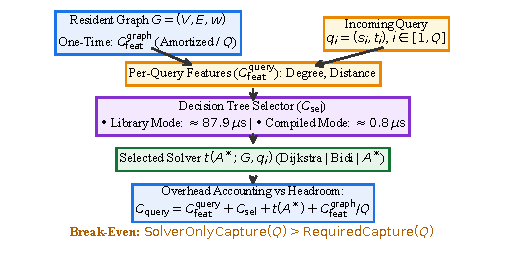
\includegraphics[width=\columnwidth]{fig1_pipeline.pdf}
\caption{Overhead-priced selection pipeline. One-time graph characterization is charged once and amortized over the workload; query features, feature-vector assembly, and selector inference recur on every query and are debited against the SBS--VBS oracle gap. Break-even requires the captured headroom to exceed the overhead fraction.}
\label{fig:pipeline}
\end{figure}

\subsection{Cost Regimes}
Two accounting regimes are reported, and they are never mixed within a single comparison. \textbf{Analysis-grade cost} combines the measured in-loop decision overhead with solver runtimes obtained under a benchmark protocol of one warm-up run followed by five timed repetitions summarized by the median; $C_{\mathrm{SBS}}$ and $C_{\mathrm{VBS}}$ use the same benchmark medians. It is a normalized cost rather than a wall-clock time, and its purpose is to remove single-shot solver timing noise, which is large at this scale (per-row relative interquartile range: median $14.39\%$, maximum $434.53\%$). \textbf{End-to-end measured cost} is the uninterrupted wall-clock runtime of the complete adaptive path, in which solver calls are timed once, as a deployment would execute them; it is reported as a supplementary physical measurement. The two regimes aggregate different timing modalities and are not expected to agree numerically. All primary comparative claims in this paper (SBS, VBS, OracleGap, CaptureRate, RequiredCapture) use the analysis-grade regime; the end-to-end measurement is reported alongside it in Section~\ref{sec:regime}.

\section{Experimental Design}

\subsection{Graphs, Queries, and Splits}
The benchmark contains 48 synthetic undirected graphs generated across three families: (1) \textbf{Erd\H{o}s--R\'enyi random} graphs with edge probability $p = D/(V-1)$ and weights drawn uniformly from $[1,100]$; (2) \textbf{random geometric} graphs with coordinates uniform in $[0,1]^2$, $k$-nearest-neighbor edges targeting average degree $D$, and metric edge weights $w(u,v) = 1.25\,\lVert u-v\rVert_2 + 0.1$; and (3) \textbf{Barab\'asi--Albert scale-free} graphs with preferential-attachment parameter $m = D/2$ and uniform weights in $[1,100]$. Each family is instantiated at $V \in \{40,80,160,320\}$ and target average degree $D \in \{6,12\}$ with two seeds per configuration, giving $3 \times 4 \times 2 \times 2 = 48$ graphs and 24 $(family,V,D)$ parameter combinations.

Table~\ref{tab:config} summarizes the configuration. The frozen split assigns 32 graphs to training, 8 to validation, and 8 to held-out testing. The eight test graphs span \emph{a subset} of the 24 parameter combinations -- three geometric, three random, and two scale-free cells; they do not cover every topology, size, and density combination, and all claims are correspondingly scoped. Queries are 500 deterministic $(s,t)$ pairs per graph, generated from a per-graph seed derived from the graph identifier and a fixed global seed, giving 24,000 queries in total. Workloads are evaluated at checkpoints $Q \in \{1,10,50,100,500\}$; each checkpoint uses the first $Q$ queries of the graph's fixed query order.

\subsection{Statistical Units and Uncertainty}
The effective independent unit of this study is the graph: the 8 held-out test graphs are the units of statistical resampling, and the 5 workload checkpoints define evaluation conditions within each graph. Consequently, the 40 graph--workload cells (8 graphs $\times$ 5 checkpoints) are \emph{evaluation conditions rather than 40 independent graph-level samples}. Uncertainty is estimated by a paired graph-level bootstrap \cite{efron1994} (1,000 replicates, fixed seed) that resamples the 8 test graphs with replacement and recomputes each metric from the paired graph-level sums; reported intervals therefore describe graph-sampling variability within the three generators, not generalization to arbitrary graph populations.

\subsection{Solver Portfolio and $A^*$ Eligibility}
The portfolio contains three exact solvers: Dijkstra's algorithm with a binary-heap priority queue; Bidirectional Dijkstra, which expands simultaneous frontiers from $s$ and $t$ and terminates when a meeting certificate closes the search; and $A^*$ with the Euclidean distance heuristic $h(u,t)=\lVert u-t\rVert_2$, memoized per $(u,t)$ pair so that repeated norm evaluations do not distort its timing. Bellman--Ford was implemented and used offline as an exactness check against all three solvers; it is not part of the online portfolio.

$A^*$ eligibility follows a conservative, metadata-driven policy. On random and scale-free graphs the coordinate embedding is not tied to the edge-weight construction, so the Euclidean heuristic carries no admissibility guarantee; $A^*$ is therefore excluded from the candidate pool for those graphs. This is a safety policy, not a claim that the heuristic is provably inadmissible there: post-hoc sampling indicated that uniform random weights frequently satisfy $h(u,t) \le d^{*}(u,t)$ by numerical coincidence, and we do not rely on that observation. Label auditing in the frozen records confirms that $A^*$ never attains the minimum eligible runtime on random or scale-free instances, so the eligibility policy does not change the VBS oracle for those cells.

\subsection{Selector Features and Decision-Time Availability}
\label{sec:features}
Features are organized into three cumulative tiers. \textbf{Tier 0} (6 features, $O(1)$) contains graph size and density ($|V|$, $|E|$, average degree), a flag indicating whether a coordinate embedding is available, and the source and target degrees. \textbf{Tier 1} (21 features) adds degree statistics (mean, variance, minimum, maximum); edge-weight statistics (mean, variance, minimum, maximum); the fraction of non-positive edges; two graph-level summaries of the edge-level geometry-to-weight ratio, $h$-ratio$(u,v)=\lVert u-v\rVert_2 \,/\, w(u,v)$, whose mean and variance serve as pre-solver proxies for how closely edge weights follow the coordinate embedding; and four query-level features (source--target Euclidean distance, that distance normalized by $\sqrt{2}$, the degree product normalized by the squared mean degree, and the degree difference). \textbf{Tier 2} (23 features) adds the average local clustering coefficient and an approximate diameter obtained by a two-sweep unweighted BFS. Tier 1 is the primary configuration; Tier 0 and Tier 2 are used for the feature-cost sensitivity analysis in Section~\ref{sec:generalization}.

All online selector features satisfy a single admissibility requirement: they must be computable before the selected solver runs. Concretely, every feature is derived from graph metadata and structure, edge weights, the coordinate embedding, and the query endpoints. No feature uses the ground-truth shortest-path distance, solver runtime, node-expansion counts, or any other post-solver information; graph-level features are computed once per resident graph, and query-level features depend only on $(s,t)$ and static graph properties. The feature set was audited against this requirement in the implementation, and the two graph-level ratio summaries are computed from edge endpoints and edge weights alone, not from any path computation.

\subsection{Selector, Training, and Deployment Modes}
The selector is a \texttt{DecisionTreeClassifier} trained on per-instance VBS labels under unweighted $0/1$ classification loss. Hyperparameters were selected on the validation split only, by grid search over the splitting criterion (Gini), maximum depth $\{2,3,4,5,6\}$, and minimum leaf size $\{1,2,3,5,10\}$; the selected configuration uses Gini, maximum depth 6, minimum leaf size 3, and produces 61 leaves. The same hyperparameters are used for every feature tier so that tier comparisons isolate the feature set rather than the model.

Two deployment modes are evaluated with identical features and identical solver implementations. \textbf{Library mode} uses the standard single-row \texttt{scikit-learn} inference path (\texttt{predict} on one instance), which is what an out-of-the-box deployment pays. \textbf{Compiled mode} evaluates the same fitted tree through nested native conditional branches generated from the tree structure, eliminating Python object wrapping and per-call array allocation. Compiled mode changes only the price of the decision; the solver choices are those of the same fitted tree.

\subsection{Timing Protocol and Noise Qualification}
\label{sec:timing}
All timing ran on an Intel 12th-generation Core processor (12 execution cores) under 64-bit Windows 11 with CPython 3.13.7 (native AMD64). Solver runtimes use one warm-up execution followed by five timed repetitions, summarized by the median and interquartile range, with \texttt{time.perf\_counter}. Micro-operations (query features, selector inference) are timed with batched execution ($B=50$) so that they exceed timer granularity. Graph features are timed once per graph and charged to the workload a single time. The adaptive path is executed over three full passes, and the pass-to-pass dispersion of the aggregate is $16.32\%$ for library inference and $9.40\%$ for compiled inference.

These dispersions define the resolution at which a difference can be called a result. A graph--workload cell is counted as a \textbf{genuine crossover} only if (i) the primary task accounting gives $C_{\mathrm{Adaptive}}(Q) < C_{\mathrm{SBS}}(Q)$ and (ii) the absolute difference is at least the empirical noise floor for the same aggregate ($16.32\%$ primary; the compiled aggregate is additionally compared against its own $9.40\%$ dispersion). Cells that satisfy (i) but not (ii) are reported as nominal and are not interpreted as wins.

\begin{table}[t]
\caption{Experimental Configuration}
\label{tab:config}
\centering
\footnotesize
\begin{tabular}{lp{4.7cm}}
\toprule
\textbf{Parameter} & \textbf{Specification / Value} \\
\midrule
Experiment ID & \texttt{\tiny stage20\_corrected\_20260923\_092749} \\
Graph families & Erd\H{o}s--R\'enyi, geometric ($k$-NN), scale-free \\
Vertex counts ($V$) & $\{40,80,160,320\}$ \\
Target average degrees ($D$) & $\{6,12\}$ \\
Graphs (24 cells) & 48 (two seeds per cell) \\
Split & 32 train / 8 validation / 8 test \\
Queries per graph & 500 deterministic $(s,t)$ pairs (24,000 total) \\
Workload checkpoints ($Q$) & $\{1,10,50,100,500\}$ \\
Portfolio & Dijkstra, Bidirectional Dijkstra, $A^*$ \\
Feature tiers & Tier 0 (6), Tier 1 (21), Tier 2 (23) \\
Selector & \texttt{DecisionTreeClassifier} (Gini, depth 6, leaf 3) \\
Timing & 1 warm-up + 5 repetitions (median); batch $B=50$ \\
Noise floors & $16.32\%$ (library), $9.40\%$ (compiled) \\
Bootstrap & $B=1{,}000$ paired graph-level resamples, 95\% CI \\
Platform & Intel 12th-Gen (12 cores), Win 11, CPython 3.13.7 \\
\bottomrule
\end{tabular}
\end{table}

\section{Results}
\label{sec:results}

\subsection{Fixed-Policy Baseline}
Cumulative benchmark-median runtimes over the 16,000 training queries select Bidirectional Dijkstra as SBS: Bidirectional Dijkstra $3.6708\,\mathrm{s}$ ($229.43\,\mu\mathrm{s}$/query), Dijkstra $6.7038\,\mathrm{s}$ ($418.99\,\mu\mathrm{s}$/query), and $A^*$ $7.6452\,\mathrm{s}$ ($477.83\,\mu\mathrm{s}$/query). Because $A^*$ is only eligible on geometric graphs, we repeated the comparison on the 5,000 training queries where all three solvers are eligible: Bidirectional Dijkstra $1.6092\,\mathrm{s}$, Dijkstra $1.9206\,\mathrm{s}$, $A^*$ $2.5516\,\mathrm{s}$. Bidirectional Dijkstra is the fixed policy on both query sets, so the SBS identity does not depend on the eligibility rule.

\subsection{Solver Complementarity}
\label{sec:complementarity}
Per-query winner shares, computed from the benchmark medians over eligible solvers, show where selection has something to exploit. On the 16 random geometric graphs, Bidirectional Dijkstra wins $37.8\%$--$66.8\%$ of queries, Dijkstra $23.4\%$--$50.4\%$, and $A^*$ $5.6\%$--$19.6\%$. On random and scale-free graphs, Bidirectional Dijkstra wins $67.2\%$--$96.8\%$ of queries and Dijkstra takes the remainder; $A^*$ is ineligible and never wins there. Meaningful solver diversity therefore exists in the geometric family, which provides measurable theoretical headroom for an adaptive selector, while the non-geometric families offer little room for improvement over the fixed policy.

\begin{table*}[t]
\caption{Workload-Amortization Economics Across Query Workloads $Q$}
\label{tab:workload_q}
\centering
\begin{tabular}{rrrrrrrrr}
\toprule
\textbf{Workload} & \textbf{SBS Cost} & \textbf{VBS Cost} & \textbf{OracleGap} & \textbf{Adaptive Cost} & \textbf{Overhead} & \textbf{CaptureRate} & \textbf{RequiredCap} & \textbf{Solver-Only} \\
$\mathbf{(Q)}$ & \textbf{(ms)} & \textbf{(ms)} & \textbf{(ms)} & \textbf{(ms)} & \textbf{(ms)} & \textbf{(task)} & \textbf{(task)} & \textbf{Capture} \\
\midrule
$Q = 1$   & 1.362    & 1.350   & 0.012   & 11.452   & 10.090  & -847.8926 & 847.8926 & 0.0000 \\
$Q = 10$  & 22.775   & 20.016  & 2.759   & 42.184   & 18.890  & -7.0353   & 6.8473   & -0.1880 \\
$Q = 50$  & 108.448  & 94.738  & 13.710  & 161.211  & 51.109  & -3.8487   & 3.7280   & -0.1207 \\
$Q = 100$ & 223.777  & 198.342 & 25.435  & 328.120  & 100.226 & -4.1024   & 3.9405   & -0.1619 \\
$Q = 500$ & 1064.200 & 941.677 & 122.523 & 1556.250 & 472.040 & -4.0160   & 3.8527   & -0.1633 \\
\bottomrule
\end{tabular}
\vspace{0.4ex}
\raggedright
\scriptsize \textit{Cost regime:} analysis-grade (measured in-loop task overhead plus benchmark-median solver runtimes), aggregated over the 8 held-out test graphs (4,000 queries at $Q=500$), library inference. Paired graph-level bootstrap 95\% confidence intervals at $Q=500$: OracleGap $[35.96, 239.08]\,\mathrm{ms}$; CaptureRate $[-11.928, -2.485]$; RequiredCapture $[2.288, 12.003]$; SolverOnlyCapture $[-0.4735, +0.0856]$; Adaptive/SBS ratio $1.462$ $[1.324, 1.734]$.
\end{table*}

\subsection{Workload Amortization and Overhead Composition}
Table~\ref{tab:workload_q} reports the analysis-grade economics across all five checkpoints, Fig.~\ref{fig:cost_vs_q} shows the corresponding cost trajectories, and Fig.~\ref{fig:req_cap} shows the RequiredCapture trajectory. At $Q=1$ a single query carries the entire one-time graph characterization, which totals $8.464\,\mathrm{ms}$ across the eight test graphs (per-graph median $0.443\,\mathrm{ms}$; the largest graph accounts for $4.290\,\mathrm{ms}$); $\mathrm{RequiredCapture}$ is then $847.89$. As $Q$ grows, the one-time term is amortized and recurring per-query costs dominate: at $Q\geq50$, $\mathrm{RequiredCapture}$ stabilizes between $3.73$ and $3.94$, and the library-mode CaptureRate remains negative at every checkpoint, reaching $-4.0160$ at $Q=500$, where adaptive execution costs $46.2\%$ more than the fixed policy.

At $Q=500$ the available headroom is $\mathrm{OracleGap}(500)=122.523\,\mathrm{ms}$, which is $11.51\%$ of the SBS cost. Library selection spends $472.040\,\mathrm{ms}$ to make its decisions, composed of $8.464\,\mathrm{ms}$ of graph features and $463.575\,\mathrm{ms}$ of recurring per-query work. The resulting ratio,
\begin{equation}
\mathrm{RequiredCapture}(500) = \frac{472.040}{122.523} = 3.8527 > 1.0,
\end{equation}
places the whole decision above the entire oracle gap: at this price, no selector -- not even one that always executes the oracle solver -- can recover the overhead.

\subsection{Library Versus Compiled Selection Economics}
\label{sec:d}
Table~\ref{tab:economics} compares library inference against the compiled decision tree at $Q=500$; Fig.~\ref{fig:economics} summarizes the same quantities visually.

\begin{table}[t]
\caption{Library Versus Compiled Selection Economics at $Q=500$}
\label{tab:economics}
\centering
\footnotesize
\resizebox{\columnwidth}{!}{%
\begin{tabular}{lrr}
\toprule
\textbf{Quantity} & \textbf{Library} & \textbf{Compiled} \\
\midrule
Median per-query inference latency & $87.9\,\mu\mathrm{s}$ & $0.8\,\mu\mathrm{s}$ \\
Inference-latency reduction & \multicolumn{2}{c}{$\approx 110\times$} \\
\midrule
Graph feature extraction (once, 8 graphs) & $8.46\,\mathrm{ms}$ & $8.51\,\mathrm{ms}$ \\
Query feature extraction (4,000 queries) & $20.78\,\mathrm{ms}$ & $14.49\,\mathrm{ms}$ \\
Feature-vector assembly (4,000 queries) & $11.49\,\mathrm{ms}$ & $9.12\,\mathrm{ms}$ \\
Selector inference (4,000 queries) & $431.30\,\mathrm{ms}$ & $3.40\,\mathrm{ms}$ \\
Total selection overhead & $\mathbf{472.04}\,\mathrm{ms}$ & $\mathbf{35.51}\,\mathrm{ms}$ \\
\midrule
Selected-solver runtime (benchmark median) & $1084.21\,\mathrm{ms}$ & $1084.21\,\mathrm{ms}$ \\
SBS baseline & $1064.20\,\mathrm{ms}$ & $1064.20\,\mathrm{ms}$ \\
Adaptive total & $1556.25\,\mathrm{ms}$ & $1119.72\,\mathrm{ms}$ \\
Net difference vs.\ SBS & $+492.05\,\mathrm{ms}$ & $+55.52\,\mathrm{ms}$ \\
\midrule
RequiredCapture & $3.8527$ & $0.2898$ \\
Realized CaptureRate & $-4.0160$ & $-0.4532$ \\
Solver-Only Capture (zero-cost selector) & $-0.1633$ & $-0.1633$ \\
Genuine crossover cells & $0/40$ & $0/40$ \\
\midrule
Physical end-to-end runtime (supplementary) & $1191.05\,\mathrm{ms}$ & --- \\
\bottomrule
\end{tabular}%
}
\vspace{0.4ex}
\raggedright
\scriptsize \textit{Cost regime:} analysis-grade, except the physical end-to-end row. Compiled mode replaces only the selector-inference charge; features and solver choices are those of the same fitted tree, which is why SolverOnlyCapture is identical. Median latencies characterize the typical per-query cost, whereas the cumulative inference rows are sums of in-loop measurements over 4,000 queries and include the right-skewed tail.
\end{table}

Compiling the decision tree into native conditional branches reduces median per-query inference latency from $87.9\,\mu\mathrm{s}$ to $0.8\,\mu\mathrm{s}$, roughly $110\times$, and cuts cumulative selector inference from $431.30\,\mathrm{ms}$ to $3.40\,\mathrm{ms}$ over the 4,000 evaluated queries. Total selection overhead falls from $472.04\,\mathrm{ms}$ to $35.51\,\mathrm{ms}$, and $\mathrm{RequiredCapture}$ drops below one:
\begin{equation}
\mathrm{RequiredCapture}(500) = \frac{35.51}{122.523} = 0.2898 < 1.0 .
\end{equation}
The implementation of the selector therefore changes the economic regime of the decision: under library inference the decision is unaffordable at any accuracy, whereas under compiled inference it needs to capture only about $29\%$ of the oracle gap to break even. Compiled adaptive execution still costs $+55.52\,\mathrm{ms}$ more than the fixed policy at $Q=500$, but that loss is now attributable to decision quality rather than to the price of deciding.

\begin{figure}[t]
\centering
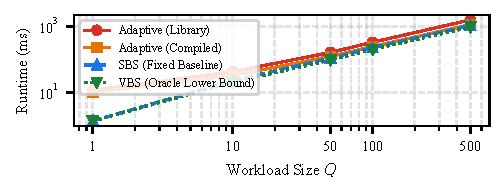
\includegraphics[width=\columnwidth]{fig2_cost_vs_q.pdf}
\caption{Cumulative execution cost versus workload size $Q$ (analysis-grade regime, log--log scale, aggregate over the 8 held-out test graphs). The library adaptive curve stays well above SBS at every checkpoint, while the compiled adaptive curve tracks closely above SBS.}
\label{fig:cost_vs_q}
\end{figure}

\begin{figure}[t]
\centering
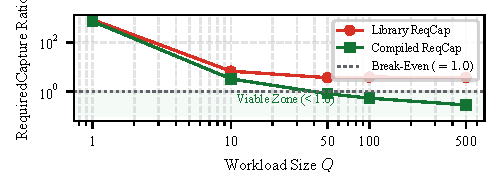
\includegraphics[width=\columnwidth]{fig3_required_capture.pdf}
\caption{RequiredCapture versus workload size $Q$. A ratio above the break-even line ($1.0$) means the decision costs more than the entire oracle gap. Library inference stays overhead-bound at every checkpoint after amortization; compiled inference enters the viable zone and reaches $0.2898$ at $Q=500$.}
\label{fig:req_cap}
\end{figure}

\begin{figure}[t]
\centering
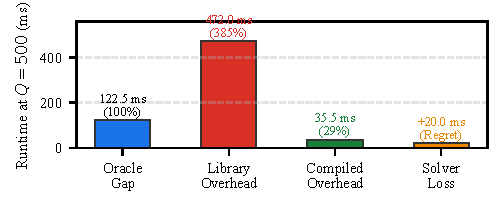
\includegraphics[width=\columnwidth]{fig4_overhead_economics.pdf}
\caption{Computational economics at $Q=500$ (analysis-grade). The oracle gap ($122.5\,\mathrm{ms}$) is the maximum saving available to any selector. Library overhead ($472.0\,\mathrm{ms}$) exceeds it by almost fourfold; compiled overhead ($35.5\,\mathrm{ms}$) is affordable but the selected solvers cumulatively cost $20.0\,\mathrm{ms}$ more than the fixed policy, so the residual limit is decision quality.}
\label{fig:economics}
\end{figure}

\subsection{Selector Efficacy and Crossover Qualification}
Because the compiled pipeline shares the solver choices of the library pipeline, the headroom it captures is the same: $\mathrm{SolverOnlyCapture}(500) = -0.1633$ with a 95\% bootstrap interval of $[-0.4735, +0.0856]$. The selected solvers cumulatively need $1084.21\,\mathrm{ms}$ against the fixed policy's $1064.20\,\mathrm{ms}$, so the decision costs $20.01\,\mathrm{ms}$ more than always running Bidirectional Dijkstra before overhead is charged. The interval includes zero, which is consistent with a selector that is, at this level of aggregation, no better than the constant policy.

Table~\ref{tab:crossover} reports the cell-level crossover audit. Under the primary task accounting, library selection produces no cell where adaptive cost falls below SBS, and compiled selection produces three nominal cells: \texttt{geometric\_V160\_D6\_s126} at $Q=500$ ($\Delta = -0.353\,\mathrm{ms}$), \texttt{random\_V80\_D12\_s108} at $Q=500$ ($\Delta = -1.486\,\mathrm{ms}$), and \texttt{scalefree\_V160\_D12\_s144} at $Q=50$ ($\Delta = -0.464\,\mathrm{ms}$). A secondary conservative sensitivity variant that excludes feature-vector assembly from the compiled overhead yields a fourth nominal cell (\texttt{random\_V40\_D6\_s102} at $Q=100$, $\Delta = -0.054\,\mathrm{ms}$; largest advantage $-2.419\,\mathrm{ms}$ at \texttt{random\_V80\_D12\_s108}, $Q=500$). Fig.~\ref{fig:per_graph_delta} shows the per-graph differences at $Q=500$.

\begin{table}[t]
\caption{Crossover Audit and Noise Qualification Across the 40 Graph--Workload Cells}
\label{tab:crossover}
\centering
\resizebox{\columnwidth}{!}{%
\begin{tabular}{lrrrr}
\toprule
\textbf{Accounting} & \textbf{Cells} & \textbf{Nominal} & \textbf{Genuine} & \textbf{Extremal cell} \\
\midrule
Library (primary) & 40 & 0 & 0 & smallest loss $+0.378\,\mathrm{ms}$ \\
Compiled (primary) & 40 & 3 & 0 & max.\ advantage $-1.486\,\mathrm{ms}$ \\
Compiled (conservative) & 40 & 4 & 0 & max.\ advantage $-2.419\,\mathrm{ms}$ \\
\bottomrule
\end{tabular}%
}
\vspace{0.4ex}
\raggedright
\scriptsize \textit{Cost regime:} analysis-grade task accounting applied identically to both modes. Noise floors: per-row benchmark-median relative interquartile range, median $14.39\%$; pass-to-pass dispersion $16.32\%$ (library) and $9.40\%$ (compiled). The largest nominal advantage ($2.419\,\mathrm{ms}$) is $0.227\%$ of the $1064.200\,\mathrm{ms}$ SBS cost, about $41\times$ below the $9.40\%$ dispersion floor.
\end{table}

These nominal advantages do not survive the resolution of the measurement environment. The largest one, $2.419\,\mathrm{ms}$, corresponds to $0.227\%$ of the SBS cost at $Q=500$, roughly $41\times$ smaller than the compiled pass-to-pass dispersion of $9.40\%$ and $72\times$ smaller than the primary $16.32\%$ floor. All three (or four, in the conservative variant) nominal cells therefore sit far below measurement resolution. Across the 40 evaluated graph--workload cells, no statistically qualified genuine crossover was observed in any mode, and the same conclusion holds under the primary and the conservative accounting.


\begin{figure}[t]
\centering
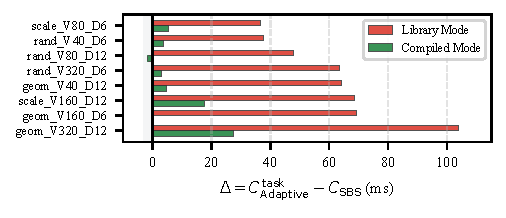
\includegraphics[width=\columnwidth]{fig6_per_graph_delta.pdf}
\caption{Per-graph runtime difference $\Delta = C_{\mathrm{Adaptive}} - C_{\mathrm{SBS}}$ at $Q=500$ (analysis-grade). All library differences are positive. The two compiled negatives ($-0.35\,\mathrm{ms}$, $-1.49\,\mathrm{ms}$) lie within the shaded band of negligible magnitude and well inside the $9.40\%$ dispersion floor of compiled execution.}
\label{fig:per_graph_delta}
\end{figure}

\subsection{Generalization and Feature-Cost Diagnostics}
\label{sec:generalization}
Table~\ref{tab:generalization} reports classification diagnostics under the held-out split and under two cross-validation protocols: leave-one-cell-out (LOCO), which holds out each $(family,V,D)$ cell in turn, and leave-one-family-out (LOFO), which holds out one graph generator.

\begin{table}[t]
\caption{Selector Generalization and Feature-Tier Economics}
\label{tab:generalization}
\centering
\resizebox{\columnwidth}{!}{%
\begin{tabular}{lrrrrr}
\toprule
\textbf{Protocol} & \textbf{Tier} & \textbf{Folds} & \textbf{Exact acc.} & \textbf{Majority} & \textbf{Constant folds} \\
\midrule
Held-out test & 1 & 1 & $72.50\%$ & $72.60\%$ & $0/1$ \\
LOCO & 0 & 24 & $79.10\%$ & $77.95\%$ & $15/24$ \\
LOCO & 1 & 24 & $80.80\%$ & $77.95\%$ & $9/24$ \\
LOFO & 0 & 3 & $83.76\%$ & $83.45\%$ & $1/3$ \\
LOFO & 1 & 3 & $79.09\%$ & $83.45\%$ & $1/3$ \\
\bottomrule
\end{tabular}%
}
\vspace{0.4ex}
\raggedright
\scriptsize \textit{Notes:} "Constant folds" counts folds in which the fitted tree predicts a single solver for every test instance. Median accuracy lift over the majority-class baseline is $+0.00$ percentage points for both LOCO protocols and for LOFO Tier 1 ($+0.06$ pp for LOFO Tier 0).
\end{table}

Classification accuracy does not measure selection quality directly, a point summarized visually in Fig.~\ref{fig:accuracy}. The held-out selector reaches $72.50\%$ exact accuracy against a $72.60\%$ majority-class baseline; median accuracy lift over the majority policy is $+0.00$ percentage points in every cross-validation protocol; and in LOCO the tree predicts a constant solver in 15 of 24 folds at Tier 0 and 9 of 24 folds at Tier 1. Under LOFO, Tier 1 accuracy ($79.09\%$) is below the majority baseline ($83.45\%$). The fitted tree does produce non-trivial predictions on the held-out split, selecting Dijkstra on a minority of queries in several cells, but the aggregate performance does not improve on the constant policy.

\begin{figure}[t]
\centering
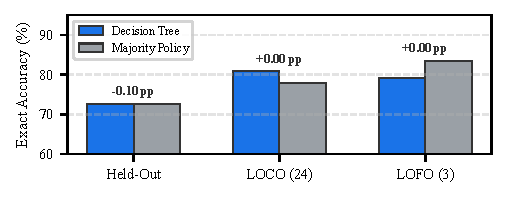
\includegraphics[width=\columnwidth]{fig5_selector_accuracy.pdf}
\caption{Exact classification accuracy of the selector against the majority-class policy for the held-out split and the Tier-1 LOCO and LOFO protocols. Accuracy differences are negligible at every protocol, which illustrates that classification accuracy is not the quantity that determines runtime viability.}
\label{fig:accuracy}
\end{figure}

The feature-cost axis behaves the same way. Raising the feature set from Tier 0 (6 features) to Tier 2 (23 features) moves held-out accuracy from $72.78\%$ to $73.30\%$, a gain of $0.52$ percentage points, while the single-pass tier sweep raises compiled RequiredCapture from $0.114$ to $0.418$: richer features cost more to compute than they return in decision quality.

\subsection{End-to-End Measurement and Regime Reconciliation}
\label{sec:regime}
Table~\ref{tab:regime} reconciles the two cost regimes at $Q=500$. The physical end-to-end run of the adaptive pipeline takes $1191.05\,\mathrm{ms}$, of which $699.87\,\mathrm{ms}$ is in-loop single-shot solver work and $491.17\,\mathrm{ms}$ is everything else the pipeline does to make and support the decision. The analysis-grade accounting of the same workload is $1556.25\,\mathrm{ms}$ = $1084.21\,\mathrm{ms}$ benchmark-median solver cost $+$ $472.04\,\mathrm{ms}$ measured decision overhead, against an SBS reference of $1064.20\,\mathrm{ms}$.

\begin{table}[t]
\caption{Cost-Regime Reconciliation at $Q=500$ (8 Test Graphs, 4,000 Queries)}
\label{tab:regime}
\centering
\resizebox{\columnwidth}{!}{%
\begin{tabular}{lrrr}
\toprule
\textbf{Regime} & \textbf{Adaptive total} & \textbf{Solver part} & \textbf{Decision part} \\
\midrule
End-to-end measured & $1191.05\,\mathrm{ms}$ & $699.87$ (single-shot) & $491.17$ \\
Analysis-grade & $1556.25\,\mathrm{ms}$ & $1084.21$ (5-rep median) & $472.04$ \\
SBS reference & $1064.20\,\mathrm{ms}$ & $1064.20$ (5-rep median) & --- \\
\bottomrule
\end{tabular}%
}
\vspace{0.4ex}
\raggedright
\scriptsize The two regimes use different solver-timing modalities and are not expected to match numerically. The decision components agree to within about $4\%$, which is the expected relationship; the solver components differ because the end-to-end pass times each solver once, as a deployment would, while the analysis-grade regime uses warm-up plus five-repetition medians.
\end{table}

The difference between $1191.05\,\mathrm{ms}$ and $1556.25\,\mathrm{ms}$ is a difference of aggregation, not a contradiction: the end-to-end figure contains single-shot solver timings, whereas the analysis-grade figure pairs the same measured decision overhead with benchmark-median solver costs so that the comparison against $C_{\mathrm{SBS}}$ uses one consistent timing modality. Because of that pairing, the primary comparative claims in this paper are made in the analysis-grade regime, and the end-to-end measurement is reported as supplementary physical evidence. Under the end-to-end regime the adaptive path remains above the $1064.20\,\mathrm{ms}$ SBS reference as well, so the qualitative conclusion does not depend on the choice of regime.

\section{Discussion}

\subsection{Finding 1: Selection Overhead Is a First-Order Cost at Microsecond Solver Runtimes}
At $Q=500$, the library pipeline spends $472.04\,\mathrm{ms}$ on its decisions over 4,000 queries, an average of $118.0\,\mu\mathrm{s}$ per query, against an average oracle headroom of
\begin{equation}
\frac{\mathrm{OracleGap}(500)}{8 \times 500} = \frac{122.523\,\mathrm{ms}}{4000} \approx 30.6\,\mu\mathrm{s}/\mathrm{query}.
\end{equation}
The decision costs about four times the maximum saving it could possibly produce. This is a structural property of the workload, not a defect of the particular tree: as long as a query runs in hundreds of microseconds and inference requires tens to hundreds of microseconds, the selector's price and the solver's variability are of the same order. The one-time graph characterization is a second-order concern that only dominates at very small $Q$ ($\mathrm{RequiredCapture} = 847.89$ at $Q=1$); from $Q=50$ onward, recurring per-query costs determine viability.

\subsection{Finding 2: Compilation Changes the Economic Regime of the Decision}
Compiling the tree to native branches lowers per-query inference from $87.9\,\mu\mathrm{s}$ to $0.8\,\mu\mathrm{s}$, which reduces the recurring decision cost to $8.9\,\mu\mathrm{s}$ per query, or $29\%$ of the available per-query headroom ($\mathrm{RequiredCapture}=0.2898$). Overhead stops being the binding constraint: a selector that captured roughly a third of the oracle gap would pay for itself. Since the solver choices are unchanged, the compiled measurement isolates the price of inference from the quality of the decision, and the comparison shows that the same policy can be economically infeasible or feasible depending only on how the decision is executed.

\subsection{Finding 3: After Overhead Is Controlled, the Objective Becomes the Bottleneck}
$\mathrm{SolverOnlyCapture}(500) = -0.1633$ with a bootstrap interval that includes zero: the chosen solvers are, in aggregate, no better than the fixed policy, and slightly worse. Two observations explain how this can hold while a decision tree is at all active. First, the training signal is a label -- the identity of the VBS solver -- and unweighted $0/1$ loss assigns the same penalty to a misprediction that costs a few microseconds and one that costs milliseconds. In this benchmark, the solvers differ by tens of microseconds on most queries and by much more on a minority; a classifier that maximizes expected accuracy need not reduce expected runtime, and here it does not. Second, the collapses observed in cross-validation (constant predictions in 9 of 24 Tier-1 LOCO folds and a below-majority LOFO result) show that the learned structure generalizes poorly across cells and families, so the small number of expensive mispredictions is not offset by systematic gains elsewhere. Capacity is not the binding issue: the same tree class reaches $72.5\%$ accuracy at depth 6, and adding features to Tier 2 moves accuracy by half a percentage point.

\subsection{Implications and Design Consequences}
The accounting framework transfers beyond this benchmark, because it compares two wall-clock quantities -- the cost of the decision and the headroom available for it -- and can therefore be instantiated in other languages and hardware, where the absolute microsecond values will differ but the ratio structure will not. Three consequences follow from the measurements, and we present them as hypotheses motivated by the results rather than as validated interventions. (i) Selection objectives should be cost-sensitive: training against runtime regret, or predicting runtime directly and dispatching to the lowest predicted mean, aligns the learning target with the quantity being optimized; whether that alignment converts the available geometric headroom into a genuine speedup is an open empirical question that this study does not settle. (ii) Deployment cost belongs in the design loop: the same decision tree moved from $3.85\times$ overhead to $0.29\times$ merely by changing how inference executes, so selector engineering should treat inference as part of the algorithm rather than an implementation detail. (iii) Headroom should be measured before selector work begins: where winner shares are as concentrated as they are on random and scale-free graphs, no selector can recover much, and effort is better directed at instances where the VBS--SBS gap is large.

\section{Limitations and Threats to Validity}

The scope boundaries below are part of the result, not caveats to it. (1) \emph{Synthetic families:} the benchmark uses Erd\H{o}s--R\'enyi, random geometric, and Barab\'asi--Albert graphs; road networks, transit networks, and power grids have structure that these generators do not reproduce. (2) \emph{Scale:} $V \le 320$; on much larger graphs both solver runtimes and winner shares change, and the oracle gap is expected to grow, which would change the break-even balance. (3) \emph{Portfolio:} three textbook solvers; preprocessing techniques such as contraction hierarchies or hub labeling are not evaluated, and their inclusion would alter both the headroom and the feature landscape. (4) \emph{$A^*$ eligibility:} a metadata-driven safety policy, not an empirical inadmissibility result; it withholds $A^*$ from two families where it never wins in any case. (5) \emph{Loss function:} the selector uses unweighted $0/1$ loss; no cost-sensitive or regret-aware variant was trained in this study, so the efficacy bottleneck is characterized, not resolved. (6) \emph{Timing environment:} CPython 3.13 on a consumer Windows machine; the absolute microsecond values are environment-specific, and only the ratio structure is expected to carry over. (7) \emph{Query model:} queries are sampled uniformly without locality or burst structure, which affects feature amortization but not the one-time/recurring decomposition. (8) \emph{Test-set size:} eight held-out graphs, covering 8 of the 24 parameter combinations, with bootstrap intervals that describe graph-sampling variability within these generators. (9) \emph{Scope of the negative result:} the finding is that no genuine crossover was observed in the evaluated cells under the primary and conservative accountings; it is not a claim of universal non-viability of adaptive shortest-path selection.

\section{Reproducibility}
\label{sec:repro}

The study is built around a frozen, version-controlled artifact set under the experiment identifier \texttt{stage20\_corrected\_20260923\_092749}. Graph generation, query generation, splitting, training, and timing are deterministic; the split is recorded in a frozen manifest, and the raw records contain 72,000 solver executions (48 graphs $\times$ 500 queries $\times$ 3 solvers) plus the adaptive records for three feature tiers and three execution passes. An automated verification script checks 15 conditions over the raw data, including partition disjointness, row counts, runtime positivity, timeout semantics, replayability of the SBS totals from the raw rows, identity of hyperparameters across tiers, and consistency between the reported values and the frozen tables. Integrity manifests record SHA-256 digests for the 75 source files of the final lock state and for the 44 audit-evidence files with an aggregate digest, together with an immutable historical baseline manifest whose 52 recorded hashes reproduce; a single pre-closure snapshot documents 166 of 167 hashes reproducing, the one divergence being a mandated reproduction-safety edit to the analysis script, which is recorded rather than hidden. The test suite contains 79 unique tests. Reproduction proceeds by running the experiment driver, the analysis script, and the verification script in sequence over the frozen configuration: \texttt{python -u scripts/run\_stage20\_}\allowbreak\texttt{corrected.py}, \texttt{python -u scripts/analyze\_corrected\_}\allowbreak\texttt{stage20.py}, and \texttt{python -u scripts/verify\_corrected\_}\allowbreak\texttt{stage20.py}.

\balance
\section{Conclusion}

This work establishes an overhead-aware methodology for deciding whether adaptive shortest-path algorithm selection can justify its own computational cost. Rather than asking whether a selector can be accurate, it asks whether the decision it makes can pay for itself out of the performance headroom that exists on the workload, and it answers that question with measured wall-clock quantities: the price of graph features, query features, vector assembly, and inference on one side, and the SBS--VBS oracle gap on the other.

The measurements expose two distinct bottlenecks. Under conventional library inference, selection is overhead-bound: at $Q=500$ the decision costs $3.8527$ times the entire available headroom, so no selector, however accurate, can break even. Compiling the decision tree into native conditional branches reduces per-query inference from $87.9\,\mu\mathrm{s}$ to $0.8\,\mu\mathrm{s}$ and moves the ratio to $0.2898$, which places selection inside the affordable region. In that second regime the bottleneck changes character: with the price of the decision no longer binding, a conventional decision-tree classifier trained under unweighted $0/1$ classification loss still fails to convert the available complementarity into solver-side savings ($\mathrm{SolverOnlyCapture} = -0.1633$), and after qualifying nominal differences against empirical measurement dispersion, none of the 40 evaluated graph--workload cells shows a genuine crossover.

Solver complementarity is present in the benchmark -- on geometric graphs $A^*$ is the per-query winner on $6\%$--$20\%$ of queries, and Dijkstra on $23\%$--$50\%$ -- so the limiting factor within this envelope is the selection objective and its generalization, not the absence of exploitable structure. The results therefore motivate runtime-regret-aware and cost-sensitive selector objectives and, more broadly, evaluation protocols that charge the decision against the headroom it is meant to exploit. These conclusions are restricted to the evaluated synthetic undirected graph families, vertex counts up to 320, the uniform random query distribution, the three-solver portfolio, and the timing environment described in Section~\ref{sec:timing}.

\begin{thebibliography}{10}

\bibitem{dijkstra1959}
E.~W. Dijkstra, ``A note on two problems in connexion with graphs,'' \emph{Numerische Mathematik}, vol.~1, no.~1, pp. 269--271, 1959.

\bibitem{bast2016}
H.~Bast, D.~Delling, A.~Goldberg, M.~M{\"u}ller-Hannemann, T.~Pajor, P.~Sanders, D.~Wagner, and R.~F. Werneck, ``Route planning in transportation networks,'' in \emph{Algorithm Engineering}, ser. LNCS, vol. 9220.\ Springer, 2016, pp. 19--80.

\bibitem{nicholson1966}
T.~A.~J. Nicholson, ``Finding the shortest route between two points in a network,'' \emph{The Computer Journal}, vol.~9, no.~3, pp. 275--280, 1966.

\bibitem{pohl1971}
I.~Pohl, ``Bi-directional search,'' in \emph{Machine Intelligence 6}, B.~Meltzer and D.~Michie, Eds.\ Edinburgh, UK: Edinburgh University Press, 1971, pp. 127--140.

\bibitem{hart1968}
P.~E. Hart, N.~J. Nilsson, and B.~Raphael, ``A formal basis for the heuristic determination of minimum cost paths,'' \emph{IEEE Transactions on Systems Science and Cybernetics}, vol.~4, no.~2, pp. 100--107, 1968.

\bibitem{rice1976}
J.~R. Rice, ``The algorithm selection problem,'' \emph{Advances in Computers}, vol.~15, pp. 65--118, 1976.

\bibitem{xu2008}
L.~Xu, F.~Hutter, H.~H. Hoos, and K.~Leyton-Brown, ``{SATzilla}: Portfolio-based algorithm selection for {SAT},'' \emph{Journal of Artificial Intelligence Research}, vol.~32, pp. 565--606, 2008.

\bibitem{hutter2014}
F.~Hutter, L.~Xu, H.~H. Hoos, and K.~Leyton-Brown, ``Algorithm runtime prediction: Methods \& evaluation,'' \emph{Artificial Intelligence}, vol. 206, pp. 79--111, 2014.

\bibitem{gebser2014}
M.~Gebser, R.~Kaminski, B.~Kaufmann, T.~Schaub, M.~Schneider, and S.~Ziller, ``claspfolio 2: Portfolio-based algorithm selection for answer set programming,'' \emph{Theory and Practice of Logic Programming}, vol.~14, no. 4-5, pp. 589--603, 2014.

\bibitem{bischl2016}
B.~Bischl, P.~Kerschke, L.~Kotthoff, M.~Lindauer, C.~Malitsky, A.~Fr{\'e}chette, H.~Hoos, F.~Hutter, K.~Leyton-Brown, K.~Tierney, and J.~Vanschoren, ``{ASlib}: A benchmark library for algorithm selection,'' \emph{Artificial Intelligence}, vol. 237, pp. 41--58, 2016.

\bibitem{kotthoff2014}
L.~Kotthoff, ``{LLAMA}: Leveraging learning to automatically manage algorithms,'' \emph{AI Communications}, vol.~27, no.~2, pp. 175--182, 2014.

\bibitem{lindauer2015}
M.~Lindauer, H.~H. Hoos, F.~Hutter, and T.~Schaub, ``{AutoFolio}: An automatically configured algorithm selector,'' \emph{Journal of Artificial Intelligence Research}, vol. 53, pp. 745--778, 2015.

\bibitem{kerschke2019}
P.~Kerschke, H.~H. Hoos, F.~Neumann, and H.~Trautmann, ``Automated algorithm selection: Survey and perspectives,'' \emph{Evolutionary Computation}, vol.~27, no.~1, pp. 3--45, 2019.

\bibitem{vanderblom2026}
K.~van~der Blom and D.~Vermetten, ``On the influence of the feature computation budget on per-instance algorithm selection for black-box optimization,'' \emph{arXiv preprint arXiv:2605.04954}, 2026.

\bibitem{gholami2026}
N.~Gholami~Shiri, V.~Krminac, B.~Djukanovi{\'c}, S.~D{\v{z}}eroski, M.~Tuba, and T.~Eftimov, ``Graph instance landscapes: When structural similarity does (not) reflect shortest-path performance,'' in \emph{Proc. IEEE Congress on Evolutionary Computation (CEC)}, 2026, arXiv:2606.18267.

\bibitem{goldberg2005}
A.~V. Goldberg and C.~Harrelson, ``Computing the shortest path: {A}* search meets graph theory,'' in \emph{Proc. 16th ACM-SIAM Symposium on Discrete Algorithms (SODA)}, 2005, pp. 156--165.

\bibitem{efron1994}
B.~Efron and R.~J. Tibshirani, \emph{An Introduction to the Bootstrap}.\ Boca Raton, FL: CRC Press, 1994.

\end{thebibliography}

\end{document}
